\chapter{System Implementation, Testing, Results, and Discussion}
\label{ch:implementation}

\section{Introduction}

This chapter presents the implementation, testing, results, and evaluation of
the EcoTrace: Intelligent Electronic Waste Recovery and Circular Economy
Management System. It explains how the system design described in
Chapter~\ref{ch:analysis-design} was translated into working software.

\begin{quote}
\small\itshape
\textbf{Note on this chapter's conformance to Chapter~\ref{ch:analysis-design}.}
Per NFR-ETH-9 (Section~\ref{sec:nfr}), this chapter distinguishes implemented
functionality from planned functionality explicitly rather than silently. Two
proposed technologies were not carried into the delivered system: \textbf{Google
Maps Platform} was not integrated -- pickup and route locations use the
\texttt{geolocator} Flutter package for on-device GPS capture, with route
grouping computed server-side using standard great-circle distance
calculations rather than a mapping-provider API. \textbf{PyTorch} was not
trained or bundled as an in-repository model -- electronic waste
classification is implemented as a pluggable external classification-provider
endpoint (configurable via \texttt{CLASSIFICATION\_AI\_URL}/
\texttt{CLASSIFICATION\_AI\_KEY}) with a deterministic, rule-based heuristic
fallback when no such provider is configured; this was a deliberate
architectural decision explained in Section~\ref{sec:classification-module}, not an
oversight. One technology was replaced with a closer functional match:
the backend was implemented in \textbf{Node.js/Express/TypeScript} rather
than FastAPI/Python -- both are RESTful, JSON-based, cloud-deployable
backend frameworks satisfying the same functional and non-functional
requirements (FR-INT-1 through FR-INT-10, NFR-COMP-4, NFR-PORT-5), and
the substitution does not change any requirement's intent. One capability was
added beyond the original proposal: a \textbf{Monime mobile-money payment
gateway} integration (Section~\ref{sec:payment-module}), collecting pickup fees
through Orange Money and Afrimoney as a first-class part of the pickup-request
workflow. All other technologies named in Chapters~\ref{ch:literature}
and~\ref{ch:analysis-design} -- Flutter, Cloud Firestore, Firebase Authentication,
Firebase Cloud Messaging, Cloudinary, and Render -- were delivered exactly as
proposed.
\end{quote}

The chapter describes the development environment, implementation
architecture, source-code organization, database configuration, authentication
process, backend services, image-management workflow, notification
services, location-capture functions, user interfaces, and deployment
procedure. It also presents the testing strategy used to evaluate the
implemented system -- functional testing, integration testing, interface
testing, security testing, and end-to-end sandbox and live-money payment
testing -- according to the evidence actually available from the completed
implementation. Screenshots, test evidence, API responses, database records,
and deployment evidence are included where available. Functions that were
fully implemented are distinguished from those that were partially
implemented or reserved for future development.

\section{Implementation Overview}

EcoTrace was implemented as a cloud-based client-server system with
cross-platform Flutter applications and a Node.js/Express/TypeScript
backend. The main implementation components are:

\begin{itemize}
  \item Flutter applications for Android, Web, and Windows
  \item An Express RESTful backend (\texttt{ecotrace-api}), written in
    TypeScript, validated with Zod
  \item A second, small FastAPI (Python) service (\texttt{ecotrace-notifications})
    responsible only for delivered-notification fan-out
  \item Cloud Firestore for structured application data
  \item Firebase Authentication for user identity management
  \item Firebase Cloud Messaging for notifications
  \item Cloudinary for electronic waste image hosting
  \item Monime for mobile-money pickup-fee payment (Orange Money, Afrimoney)
  \item Render for hosting both backend services
  \item Firebase Hosting for the deployed Web build
\end{itemize}

The Flutter applications provide the presentation layer and interact with
the backend both through HTTP requests to \texttt{ecotrace-api} (for
anything requiring server-side validation, business rules, or a third-party
integration) and, for specific real-time-critical reads, directly against Cloud
Firestore through authenticated listeners governed by Firestore Security
Rules -- most notably the Monime payment-status screen, which watches its
own transaction document rather than polling. The Express backend validates
requests, applies business rules, communicates with cloud services, and
returns JSON responses. Cloud Firestore stores user profiles, electronic waste
records, pickup requests, assignments, notifications, payment transactions,
and other structured system data. Images are uploaded directly from the
Flutter client to Cloudinary using a short-lived signed upload credential
issued by the backend, rather than proxied through the backend itself.

\subsection{Implemented, Partially Implemented, and Planned Features}

To ensure accurate reporting, system functions are classified using the
following implementation statuses, consistent with the definitions proposed in
Chapter~\ref{ch:analysis-design}: \textbf{Fully implemented} (developed,
integrated, and successfully exercised during testing, including against real
external services); \textbf{Partial} (a substantial, working implementation
exists, but one or more production-readiness items remain -- e.g., a
provider-configuration step outside the codebase); \textbf{External setup
required} (code exists and works, but a third-party provider account, store
listing, or cloud configuration step must still be completed by the project
owner); \textbf{Not implemented} (remains part of the originally proposed
design but was not built).

Table~\ref{tab:module-status} reports this status for every major module,
based on the module-by-module implementation audit maintained alongside
the source code (\texttt{docs/module-implementation-audit.md}) together with
the specific end-to-end testing performed on the payment module during this
project (Section~\ref{sec:testing}).

\begin{longtable}{@{}p{3.6cm}p{2.4cm}p{7.2cm}@{}}
\caption{Implementation Status of Major EcoTrace Modules} \label{tab:module-status} \\
\toprule \textbf{Module} & \textbf{Status} & \textbf{Evidence / Remaining Work} \\ \midrule
\endfirsthead
\toprule \textbf{Module} & \textbf{Status} & \textbf{Evidence / Remaining Work} \\ \midrule
\endhead
Authentication and identity & Partial & Firebase Authentication live for email/password sign-in across all roles; social-provider configuration, phone verification, and MFA enrollment remain. \\
Users and organizations & Partial & API-backed organization, approval, document, branch, invitation, and staff-role workflows implemented; emulator integration tests remain. \\
Pickup requests & Partial & Server fee estimation, required Cloudinary photos, drafts/confirmation, GPS capture, scheduling, cancellation/rescheduling, and ratings implemented and tested; payment is now a required gate before submission (Section~\ref{sec:payment-module}). \\
Payment (Monime mobile money) & \textbf{Fully implemented and live-tested} & Orange Money and Afrimoney payment-code creation, webhook-triggered confirmation, real-time Firestore-backed status UI, and a real live-money transaction were all verified working; see Section~\ref{sec:payment-module} and Section~\ref{sec:testing}. \\
Inventory & Partial & Registration, Cloudinary images, editing, location/status history, QR lookup, and batch lifecycle implemented; production barcode-label printing validation remains. \\
Classification & Partial / external setup & Manual and assisted classification, validation, review queue, and notifications implemented; the assisted path uses a pluggable heuristic-fallback classifier, not a trained PyTorch model (Section~\ref{sec:classification-module}). \\
QR traceability & Partial & QR/barcode labels, scanning, hashed custody events, and audits implemented; physical-printer acceptance testing remains. \\
Scheduling and dispatch & Partial & Schedule creation, GPS-based grouping, availability/capacity/conflict checks, and state transitions implemented; deployed push-delivery verification remains. \\
Fleet & Partial & Vehicle registration, driver assignment, inspections, maintenance, and analytics implemented; telematics integration remains. \\
Routing and GPS & Partial / external setup & GPS-based route generation, ordered stops, and tracking implemented using \texttt{geolocator}; a production roads/traffic provider (originally proposed as Google Maps Platform) was not integrated. \\
Collection centres & Partial & Registration, directory, check-in/out, storage, staffing, and capacity alerts implemented; physical scanner/scale acceptance remains. \\
Repair and refurbishment & Partial & Assessment, technician assignment, diagnosis, status transitions, parts, quality testing, and warranty implemented; emulator lifecycle tests remain. \\
Recycling & Partial & Batch creation, staged transitions, mass-balance validation, and certificates implemented; certified-facility integration remains. \\
Resource recovery & Partial & Recovered-material recording, buyer assignment, and sales ledger implemented; downstream settlement acceptance testing remains. \\
Hazardous waste & Partial & Identification, classification, incident holds, and disposal accounting implemented; licensed-facility registry integration remains. \\
Reverse logistics & Partial & Transfer creation, custody events, and exception handling implemented; route-provider integration remains (see Routing and GPS). \\
Partners and vendors & Complete & Registration, licensing, contracts, compliance, and analytics fully API-backed. \\
Marketplace & Complete & Listings, quotations, orders, payment submission, delivery tracking, and reviews fully API-backed. \\
Donations & Complete & Beneficiary registration, requests, allocation, delivery, and impact reporting fully API-backed. \\
Rewards & Complete & Wallets, redemptions, levels, and fraud checks fully API-backed. \\
Billing (admin) & Partial & Confirmation, refund, and invoicing endpoints implemented and now include a \texttt{refundPending} state triggered automatically when a paid pickup is cancelled. \\
Environmental impact & Partial & Impact calculation implemented; formula/methodology validation remains. \\
Analytics and reporting & Partial & Dashboards implemented; production PDF/XLSX export and large-data performance testing remain. \\
Notifications & Partial / external setup & In-app and event-driven notifications implemented via a dedicated FastAPI microservice; production FCM/SMS/email provider configuration remains. \\
Support, compliance, incidents, documents, audit trail, administration & Partial & API-backed across all listed modules; remaining work is integration-test coverage, not missing functionality. \\
\bottomrule
\end{longtable}

\section{Development Environment}

The EcoTrace development environment consisted of the software tools,
frameworks, cloud platforms, and devices required to build, test, and deploy
the system.

\subsection{Development Computer}
The project was developed on a Windows computer (Windows 11 Pro,
build 10.0.22631). \textit{[TO BE VERIFIED: exact processor model, installed
memory, storage type/capacity, and display resolution -- copy these from the
computer's system-information interface rather than estimating, per the
original chapter's own instruction not to invent hardware specifications.]}

\subsection{Frontend Development Environment}
Flutter and Dart were used to implement the EcoTrace client applications
for Android, Web, and Windows from a shared codebase. Visual Studio Code
(with the Flutter/Dart extensions) was the principal editor. The exact Flutter
and Dart versions in the final build are recorded by running
\texttt{flutter\ --version} in the project root; the full toolchain report is
available via \texttt{flutter\ doctor\ -v}.

\subsection{Backend Development Environment}
The primary backend (\texttt{ecotrace-api}) was implemented in TypeScript
on Node.js 22, using Express~5 for routing, Zod for request validation, and
the Firebase Admin SDK for privileged Firestore/Auth access
\citep{express2026,firebase2026admin}. A second, small backend
(\texttt{ecotrace-notifications}) was implemented in Python using FastAPI,
scoped narrowly to receiving internal event calls from \texttt{ecotrace-api} and
fanning them out to FCM/SMS/email. TypeScript is compiled with \texttt{tsc};
\texttt{npm} manages dependencies for both the client and \texttt{ecotrace-api},
while \texttt{pip} with \texttt{requirements.txt} manages the Python
notification service.

\subsection{Cloud Services and External Platforms}

\textbf{Cloud Firestore} is the primary structured-data store, with Security
Rules enforcing ownership- and role-based access independently of the API
layer. \textbf{Firebase Authentication} handles account registration, login, and
identity tokens. \textbf{Firebase Cloud Messaging} delivers workflow
notifications via the \texttt{ecotrace-notifications} service. \textbf{Cloudinary}
stores uploaded images; the client uploads directly to Cloudinary using a
short-lived signature issued by \texttt{ecotrace-api}, so the Cloudinary API
secret is never shipped to the client and large image bodies never transit the
Render-hosted backend. \textbf{Monime} \citep{monime2026} is the mobile-money
payment aggregator used for pickup-fee collection, detailed in
Section~\ref{sec:payment-module}. \textbf{Render} hosts both backend services
as free-tier Web Services, each exposing a public HTTPS endpoint and a
\texttt{/health} check; a free service may enter an inactive state after a period
without inbound requests, producing a longer response time (in practice,
observed up to roughly a minute) on the first request after inactivity, which
the Flutter API client's retry/backoff logic is written to tolerate.
\textbf{Firebase Hosting} serves the compiled Flutter Web build.

\subsection{Version Control and Repository Management}
Git was used to track project changes, with GitHub providing remote
repository hosting and triggering Render's auto-deploy on every push to the
tracked branch. Sensitive credentials, service-account files, and build outputs
are excluded from the repository via \texttt{.gitignore}; all runtime secrets
(Firebase service-account key, Monime access token, Cloudinary API secret,
CORS allow-list) are supplied to the deployed services exclusively through
Render's environment-variable configuration, never committed to source
control.

\section{Project Source-Code Organization}

The EcoTrace repository is organized into a Flutter client at the repository
root, an Express backend under \texttt{functions/}, and a separate FastAPI
notification service under \texttt{notifications\_service/}:

\begin{verbatim}
wastemanagementsystem/
|-- lib/
|   |-- main.dart
|   |-- app.dart
|   |-- firebase_options.dart
|   |-- core/
|   |   |-- api/            (ApiClient, API_BASE_URL config)
|   |   |-- app_currency.dart
|   |   `-- media/          (Cloudinary upload service)
|   `-- features/           (30 feature modules, each with
|                             domain/ data/ presentation/)
|       |-- auth/  pickups/  payments/  marketplace/
|       |-- inventory/  repairs/  recycling/  ...
|       `-- workspace/      (role-based navigation shell)
|
|-- functions/               (ecotrace-api, Node/Express/TypeScript)
|   |-- src/
|   |   |-- app.ts           (Express app, CORS, middleware)
|   |   |-- routes.ts        (mounts ~29 domain route modules)
|   |   |-- auth.ts          (authenticate, requireRoles)
|   |   |-- errors.ts        (ApiError, errorHandler)
|   |   |-- firebase.ts      (Admin SDK init)
|   |   |-- push-events.ts   (publishNotificationEvent)
|   |   |-- monime-client.ts (Monime API client)
|   |   |-- payment-routes.ts
|   |   |-- pickup-routes.ts
|   |   `-- ...              (one *-routes.ts file per domain)
|   `-- package.json
|
|-- notifications_service/   (ecotrace-notifications, FastAPI/Python)
|   |-- app/
|   `-- requirements.txt
|
|-- firestore.rules
|-- storage.rules
|-- firebase.json
|-- render.yaml
`-- pubspec.yaml
\end{verbatim}

This structure differs from the illustrative layout in
Chapter~\ref{ch:analysis-design} chiefly in two respects: the client uses a
feature-module structure (\texttt{lib/features/<domain>/\allowbreak
\{domain,data,presentation\}}) rather than a single flat
\texttt{screens}/\texttt{models}/\texttt{services} split, and the backend is an
Express/TypeScript project under \texttt{functions/} rather than a Python
\texttt{backend/} directory -- both organizational choices, not functional
differences.

\section{Frontend Implementation}

\subsection{Flutter Project Structure}
Each of the 30 feature modules under \texttt{lib/features/} follows the same
internal shape: \texttt{domain/} for plain Dart models, \texttt{data/} for the
repository layer (wrapping either \texttt{ApiClient} calls or direct Firestore
access), and \texttt{presentation/} for screens and widgets. This consistent
shape was applied across authentication, pickups, payments, marketplace,
inventory, repairs, recycling, recovery, hazardous waste, reverse logistics,
rewards, donations, notifications, and every other domain area, so that a
developer already familiar with one feature module can navigate any other.

\subsection{Application Entry Point}
The Flutter application begins execution in \texttt{lib/main.dart}, which
initializes Flutter bindings, initializes Firebase (optionally connecting to
local emulators when built with \texttt{USE\_FIREBASE\_EMULATORS=true}),
and hands off to \texttt{EcoTraceApp} once ready -- showing a branded
loading screen with retry-on-error handling in the meantime:

\begin{verbatim}
void main() {
  WidgetsFlutterBinding.ensureInitialized();
  runApp(const _EcoTraceBootstrap());
}

class _EcoTraceBootstrapState extends State<_EcoTraceBootstrap> {
  Future<void> _initialize() async {
    try {
      if (Firebase.apps.isEmpty) {
        await Firebase.initializeApp(
          options: DefaultFirebaseOptions.currentPlatform,
        );
      }
      await _connectToFirebaseEmulators();
      if (mounted) setState(() => _ready = true);
    } catch (error) {
      if (mounted) setState(() => _error = error);
    }
  }
  ...
}
\end{verbatim}

Routing itself is not name-based; \texttt{AuthGate} (in
\texttt{lib/features/auth/}) listens to Firebase Auth state and the user's
Firestore profile, and hands control to \texttt{role\_workspace\_screen.dart},
which resolves the correct \texttt{ApplicationInterface} and destination list for
the signed-in role (Section~\ref{sec:system-architecture}) and builds the
matching dashboard and navigation.

\subsection{Core Client Services}
\texttt{lib/core/api/api\_client.dart} wraps \texttt{package:http} with
automatic Firebase ID-token attachment, 401-triggered token refresh and
retry, exponential-backoff retry tuned for Render's free-tier cold starts, and
typed \texttt{get}/\texttt{getList}/\texttt{post}/\texttt{patch}/\texttt{delete}
helpers raising a typed \texttt{ApiException} on failure.
\texttt{lib/core/media/cloudinary\_upload\_service.dart} requests a signed
upload credential from the backend, then uploads the image bytes directly to
Cloudinary. \texttt{lib/core/app\_currency.dart} formats every monetary value
in the app as Sierra Leone Leone (\texttt{SLE}/\texttt{Le}).

\section{Backend Implementation}

\texttt{ecotrace-api} is an Express~5 application (\texttt{functions/src/app.ts})
composed of roughly 30 domain route modules (\texttt{*-routes.ts}), each
exporting an Express \texttt{Router} mounted in \texttt{routes.ts} under
\texttt{/api/v1}. Three cross-cutting pieces are shared by every route:

\begin{itemize}
  \item \textbf{\texttt{auth.ts}} -- the \texttt{authenticate} middleware
    verifies the caller's Firebase ID token, loads their Firestore profile, and
    rejects suspended/disabled accounts; \texttt{requireRoles(...roles)} then
    gates individual routes by role.
  \item \textbf{\texttt{errors.ts}} -- a single \texttt{ApiError} class and
    \texttt{errorHandler} middleware turn a Zod validation failure into a 400,
    an \texttt{ApiError} into its declared status, and anything else into a 500
    with no internal detail leaked to the client.
  \item \textbf{\texttt{firebase.ts}} -- initializes the Firebase Admin SDK
    once from a base64-encoded service-account secret, cross-checked against
    the expected project ID before use.
\end{itemize}

Request validation throughout the backend uses Zod schemas parsed at the
top of each handler, so a malformed request is rejected before any business
logic runs. CORS is a single app-wide middleware
(\texttt{API\_ALLOWED\_ORIGINS}, always permitting \texttt{localhost} for
local development) applied ahead of every route, so no individual endpoint
can be accidentally left open to arbitrary origins. \texttt{push-events.ts}
exposes \texttt{publishNotificationEvent()}, a best-effort POST to
\texttt{ecotrace-notifications} covering roughly 40 distinct event types used
across every domain module -- pickup, repair, recycling, hazardous, logistics,
marketplace, donation, reward, payment, compliance, fleet, and more.

\section{Database Implementation}

Cloud Firestore is used exactly as designed in
Section~\ref{sec:system-design}: as a document database with per-collection
Security Rules. Every collection's access rule follows one of a small number
of composable patterns defined once in \texttt{firestore.rules}: \texttt{owns()}
(request.auth.uid matches a document's owner field), \texttt{hasRole()}
(reads the caller's role from their own \texttt{/users/\{uid\}} document, so an
administrator's role change takes effect immediately without the affected
user needing to sign out), and, for a few collections
(\texttt{pickupRequests}, \texttt{supportTickets}), explicit
state-machine constraints on which fields can change and from which prior
status. The file ends with a deny-by-default catch-all
(\texttt{match~/\{document=**\}~\{~allow~read,~write:~if~false;~\}}), so a
collection is completely inaccessible until a rule is deliberately written for it
-- this is not a formality behind the API, since several screens (most notably
the Monime payment-status screen) read Firestore directly.

\section{Authentication and Authorization}

Firebase Authentication issues the ID token; the backend never re-implements
password handling. On the client, \texttt{AuthGate} listens for auth-state
changes and loads the matching \texttt{/users/\{uid\}} profile, which carries
the user's \texttt{role} -- one of eleven values (household, business,
institution, collector, driver, collectionCentreOperator, repairTechnician,
recycler, administrator, environmentalOfficer, superAdministrator). On the
backend, every protected route runs through \texttt{authenticate} then, where
appropriate, \texttt{requireRoles(...)}; Firestore Security Rules independently
re-derive and check the same role for any request that reaches Firestore
directly, so authorization is never enforced in only one place.

\section{Pickup Request Module}
\label{sec:pickup-module}

A pickup request is created as a \texttt{draft} the moment a citizen submits
category, quantity, a required Cloudinary photo, estimated weight, condition,
location, and a preferred date/time, with an optional urgent flag. The server
independently computes the pickup fee from this same data
(\texttt{POST~/payments/fees/calculate}) -- the client never supplies a
trusted amount. The draft cannot progress to \texttt{submitted} until its
pickup-fee payment is confirmed (Section~\ref{sec:payment-module}); from
there it follows the state machine defined in
Table~\ref{tab:pickup-states-impl}, matching the design in
Section~\ref{sec:system-design}.

\begin{table}[H]
\centering
\small
\caption{Implemented Pickup Request State Transitions}
\label{tab:pickup-states-impl}
\begin{tabular}{@{}p{2.6cm}p{9.6cm}@{}}
\toprule
\textbf{State} & \textbf{Allowed next states} \\
\midrule
draft & submitted, cancelled \\
submitted & approved, cancelled, failed \\
approved & assigned, cancelled, failed \\
assigned & scheduled, cancelled, failed \\
scheduled & inProgress, cancelled, failed \\
inProgress & collected, failed \\
collected & completed \\
failed & submitted, cancelled \\
cancelled / completed & (terminal) \\
\bottomrule
\end{tabular}
\end{table}

Cancelling a pickup that has already been paid does not silently leave the
payment record \texttt{confirmed} with no trace of the obligation -- the
backend automatically transitions the associated payment transaction to
\texttt{refundPending} (Section~\ref{sec:payment-module}), since Monime's
API exposes no refund endpoint and the actual money movement has to
happen as a manual Payout from the Monime dashboard.

\section{Payment Module -- Monime Mobile Money Integration}
\label{sec:payment-module}

This is the most extensively tested module in the system: every claim in
this section was verified against Monime's real sandbox API (and, briefly,
against a real live-money transaction), not assumed from documentation
alone. It was also added to the project after the design in
Chapter~\ref{ch:analysis-design} was written, once pickup-fee collection was
identified as a prerequisite for a pickup request to be considered complete.

\subsection{Choice of Integration Primitive}
Monime \citep{monime2026} offers two ways to collect a mobile-money
payment: a \textbf{Checkout Session}, which redirects the customer to a
Monime-hosted page, and a \textbf{Payment Code}, a short-lived,
provider-restricted USSD code the customer dials on their own phone with no
redirect at all. EcoTrace uses Payment Code, because the requirement was an
in-app provider picker and phone-number form rather than a browser
hand-off, and because Payment Code's webhook events are fully documented
with real example payloads, whereas Checkout Session's webhook events
were marked ``coming soon'' in Monime's own documentation at the time of
integration.

\subsection{End-to-End Flow}
\begin{enumerate}[leftmargin=1.4cm]
  \item The citizen fills in the pickup request and taps \textbf{Continue to
    payment}; the pickup is created as a \texttt{draft}.
  \item \texttt{POST~/payments/monime/initiate} re-derives the fee from the
    stored pickup record (never from the client), and de-duplicates: a
    repeated call for the same pickup while a payment attempt is already
    \texttt{pending} or \texttt{processing} returns the existing attempt instead
    of creating a second Monime payment code, so a double-tap can never
    double-charge.
  \item The backend calls Monime's \texttt{POST~/v1/payment-codes},
    restricting the code to the citizen's chosen provider
    (\texttt{authorizedProviders}), with a 30-minute expiry and the internal
    transaction ID as Monime's \texttt{reference}.
  \item The citizen dials the returned USSD code on their own phone; the app
    displays it with a short note that it comes from Monime and is unique to
    this payment, since it does not resemble the citizen's regular
    Orange~Money/Afrimoney menu code.
  \item Monime calls \texttt{POST~/payments/monime/webhook}
    (deliberately unauthenticated -- Monime, not an app user, calls it) once the
    payment resolves.
  \item The webhook handler treats the delivery only as a trigger: rather than
    trust the payload Monime sent, it calls back to Monime's own
    \texttt{GET~/v1/payment-codes/\{id\}} for the authoritative status before
    writing anything to Firestore.
  \item The payment transaction is updated to \texttt{confirmed} or
    \texttt{failed}; if it was a pickup fee, \texttt{confirmPickupAfterPayment()}
    (in \texttt{pickup-routes.ts}) auto-advances the draft pickup to
    \texttt{submitted}.
  \item The Flutter payment screen, which has been watching that transaction
    document via a Firestore \texttt{.snapshots()} listener since step~2, updates
    itself the instant step~7 writes -- no polling.
\end{enumerate}

\subsection{Two Real, Undocumented Monime API Bugs}
Both of the following were discovered only by reproducing them against the
live sandbox, not by reading Monime's published OpenAPI schema, which
documents neither.

\begin{quote}
\small
\textbf{Provider and phone number are mutually exclusive.} Setting both
\texttt{authorizedProviders} and \texttt{authorizedPhoneNumber} on the same
Payment Code request returns \texttt{400 arguments\_invalid} (``A payment
provider must not be set when a paying phone number is specified''). EcoTrace
restricts by provider only. Monime's own USSD Simulator (its sandbox testing
tool) can only simulate one fixed test number per network, so a
phone-restricted code could never have been completed through Monime's
own test tooling regardless. The phone number the citizen enters is still
collected and stored on the transaction record for the receipt; it is simply not
sent to Monime as an enforcement restriction.
\end{quote}

\begin{quote}
\small
\textbf{Webhook creation is blocked entirely while a Monime Space is in
Test Mode} -- both via the API (\texttt{403}) and the dashboard UI (the Create
Webhook control is disabled). A webhook must be registered while the
dashboard is toggled to Live Mode, even though it can still receive
test-environment event deliveries afterward.
\end{quote}

\subsection{Provider Mapping}
\begin{table}[H]
\centering
\caption{Monime Mobile Money Provider Mapping}
\label{tab:monime-providers}
\begin{tabular}{@{}p{3cm}p{3cm}p{6.5cm}@{}}
\toprule
\textbf{App value} & \textbf{Monime ID} & \textbf{Network} \\
\midrule
orangeMoney & m17 & Orange Money Sierra Leone \\
afrimoney & m18 & Afrimoney \\
\bottomrule
\end{tabular}
\end{table}

Q-Money -- requested alongside Orange Money and Afrimoney during
requirements discussions -- was confirmed, via a live call to Monime's own
\texttt{GET~/v1/momos} provider-listing endpoint, not to be a Monime-supported
provider. It was never implemented, rather than implemented incorrectly.

\subsection{Security Properties, As Tested}
\begin{itemize}
  \item The charged amount is always server-recomputed from the pickup's
    own stored data; the amount shown in the Flutter form is read-only.
  \item The webhook handler never trusts Monime's payload directly -- see
    step~6 above -- which matters concretely because Monime's
    \texttt{Monime-Signature} webhook-signature construction is undocumented
    and could not be reverse-engineered even after testing it against three
    independently captured real deliveries with a freshly copied, verified
    secret, following every standard convention (Stripe-style, Slack-style,
    Svix-style) and checking Monime's own open-source \texttt{monime-cli}
    tooling for a reference implementation. The re-fetch-from-API pattern is a
    genuine mitigation for this gap, not a full substitute for signature
    verification, and is flagged here rather than glossed over.
  \item No Monime credential (\texttt{MONIME\_ACCESS\_TOKEN},
    \texttt{MONIME\_SPACE\_ID}) appears anywhere in the Flutter source or the
    built Web output -- verified directly by grepping both.
  \item Monime's Payment Code API exposes no way to detect an
    insufficient-funds failure as a distinct event -- a failed attempt simply
    leaves the code \texttt{pending}, observationally identical to ``no attempt
    yet.'' The app compensates with a client-side timeout (three minutes)
    that then offers a retry with an honest, approximate explanation, rather
    than claiming a precise diagnosis it cannot actually make.
\end{itemize}

\section{Collection, Logistics, Repair, Recycling, and Marketplace Modules}
These modules follow the API-backed, Firestore-persisted pattern described
above: authenticated Express routes validate input with Zod, enforce role and
ownership, write to the collections defined in
Section~\ref{sec:system-design}, and publish notification events on every
significant transition. Their functional coverage is summarized in
Table~\ref{tab:module-status}; none required a materially different
architecture from what Chapter~\ref{ch:analysis-design} proposed.

\section{Notification Module}
Every significant workflow transition across every module calls
\texttt{publishNotificationEvent()}, which POSTs to the separate
\texttt{ecotrace-notifications} FastAPI service with a shared secret header
(\texttt{x-ecotrace-event-key}). That service is intentionally the only part of
the system still built on FastAPI/Python -- a deliberate, narrow use of the
originally proposed backend framework for a small, well-isolated
responsibility, rather than a partial migration left incomplete.

\section{Dashboards and Reporting}
Each of the four \texttt{ApplicationInterface} groups (citizen,
fieldOperations, processing, administration --
Section~\ref{sec:system-architecture}) has its own dashboard widget, populated
from role-scoped API/Firestore queries. Administrative reporting
(\texttt{report-routes.ts}, \texttt{analytics-routes.ts}) supports filtering by
date, status, category, and location as designed; production PDF/XLSX export
and large-dataset performance testing remain open items, as reported
honestly in Table~\ref{tab:module-status}.

\subsection{Electronic Waste Classification Module}
\label{sec:classification-module}
Classification is implemented as a pluggable external provider: if
\texttt{CLASSIFICATION\_AI\_URL} and \texttt{CLASSIFICATION\_AI\_KEY} are
configured, the backend forwards the image to that endpoint; if not, it falls
back to a deterministic, rule-based heuristic. This was a deliberate design
choice, made once it became clear that training and hosting a bespoke
PyTorch model was a substantially larger undertaking than the rest of the
project's scope justified, and that keeping the AI provider pluggable behind a
stable interface (rather than hard-wiring a specific framework) satisfies
NFR-SCAL-8 (``the AI service shall allow replacement or upgrading of the
selected model without redesigning the complete client application'') more
directly than shipping an unvalidated first model would have.

\section{User Interface Screens}

\begin{figure}[H]
  \centering
  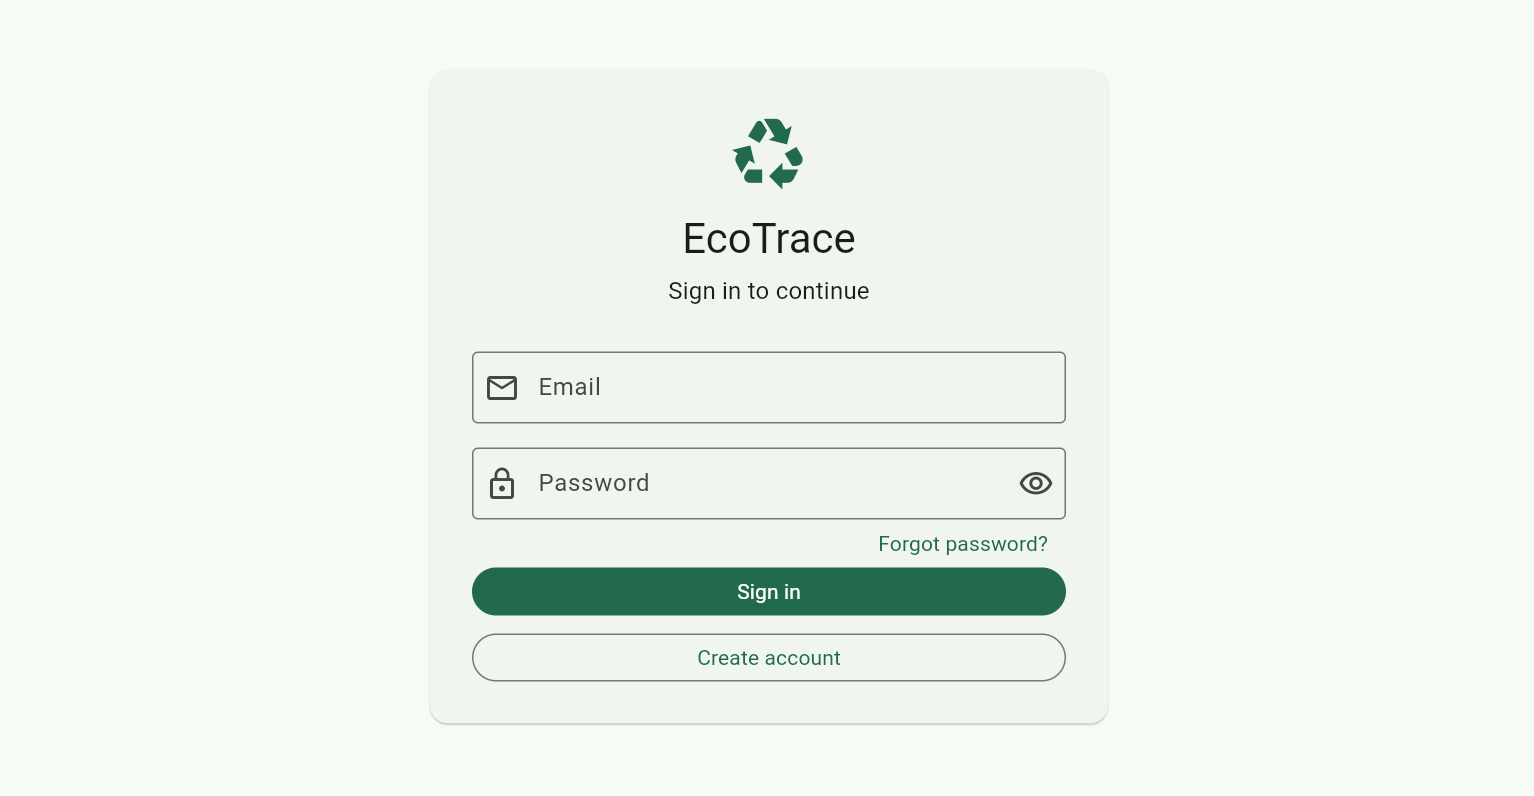
\includegraphics[width=0.55\textwidth]{figures/login-screen.png}
  \caption{Login Screen}
  \label{fig:screen-login}
\end{figure}

\begin{figure}[H]
  \centering
  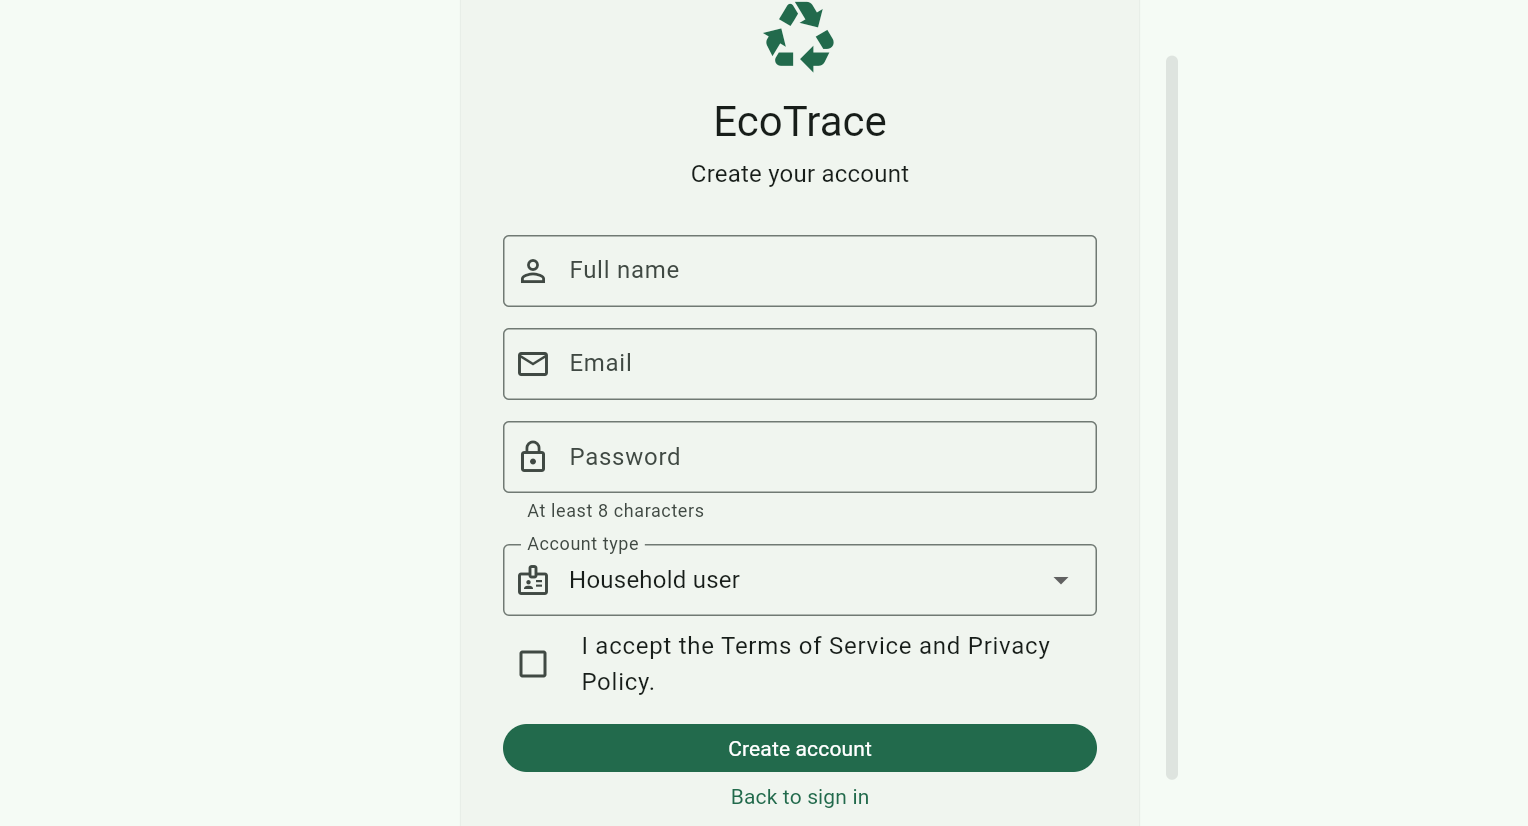
\includegraphics[width=0.55\textwidth]{figures/registration-screen.png}
  \caption{Registration Screen}
  \label{fig:screen-registration}
\end{figure}

\begin{figure}[H]
  \centering
  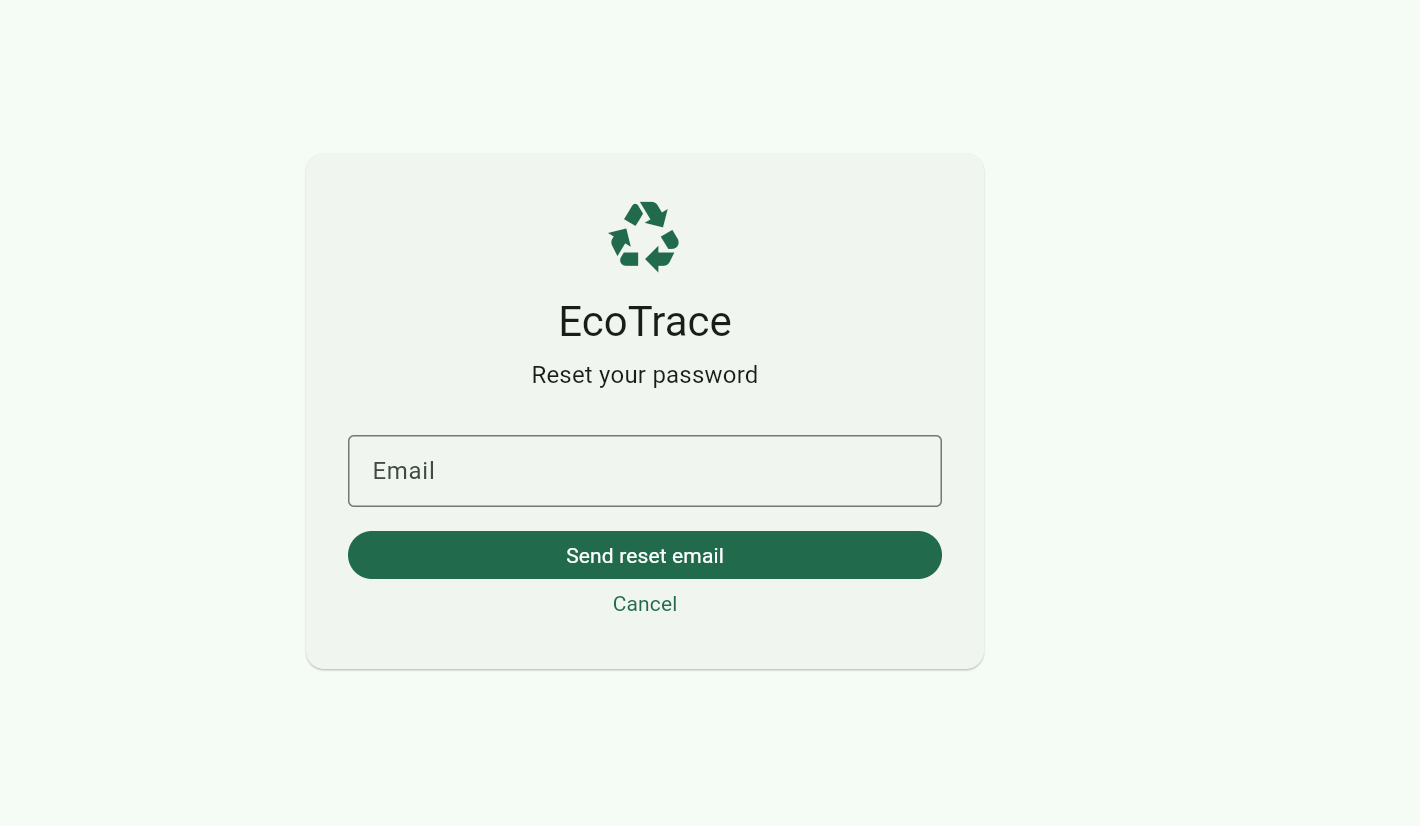
\includegraphics[width=0.55\textwidth]{figures/forgot-password-screen.png}
  \caption{Forgot Password (Reset Password) Screen}
  \label{fig:screen-forgot-password}
\end{figure}

\begin{figure}[H]
  \centering
  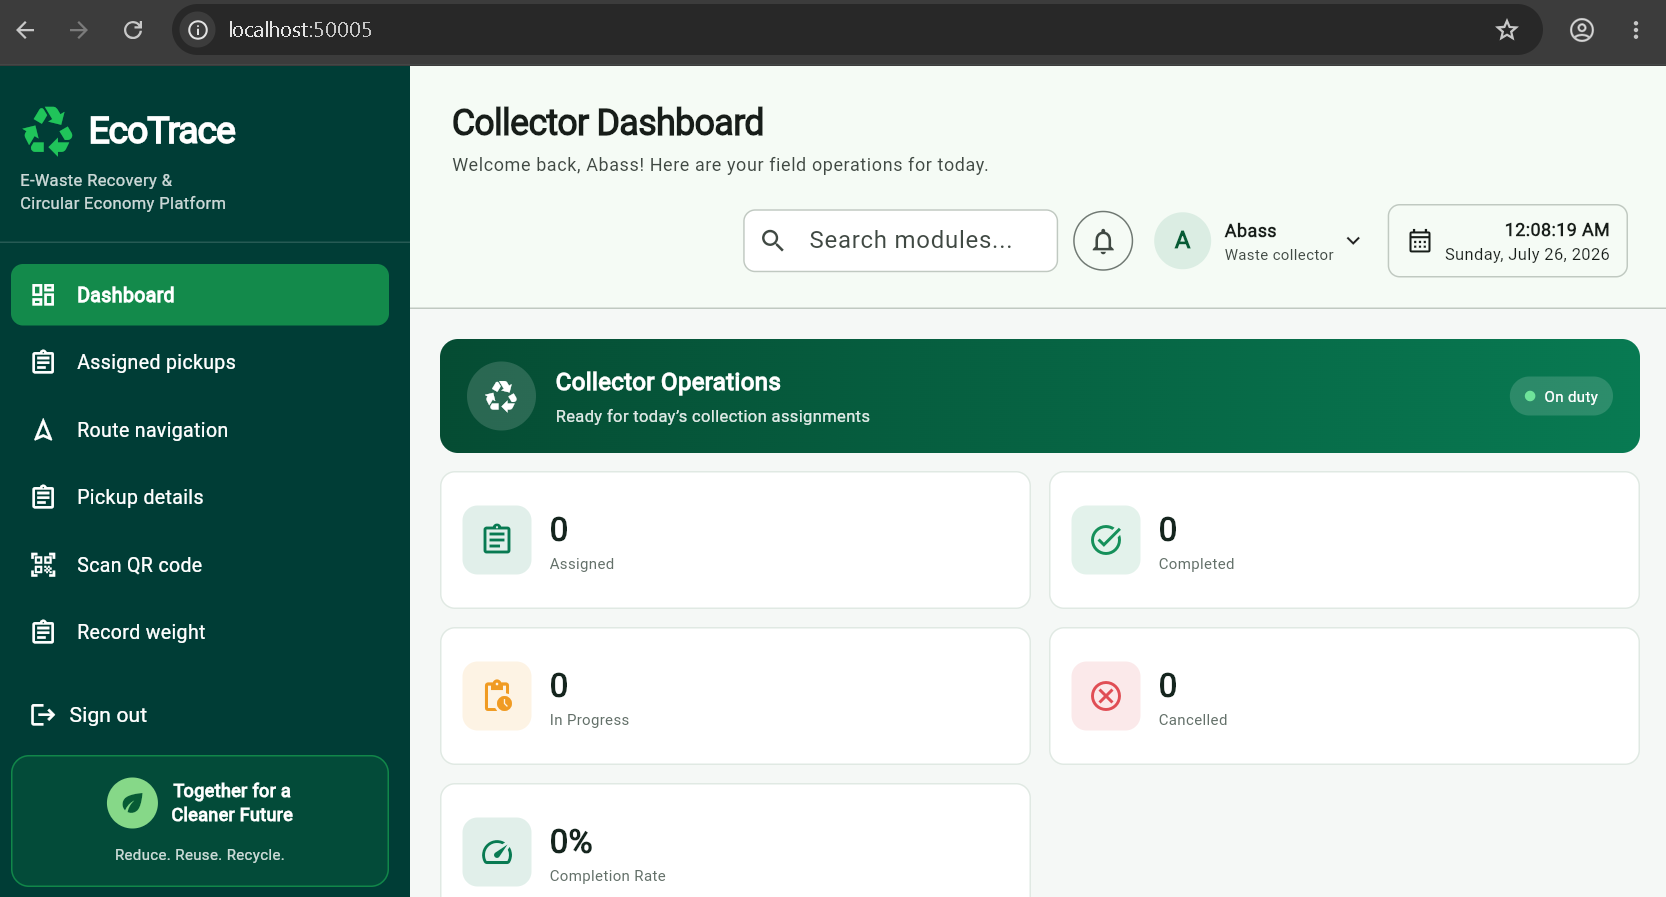
\includegraphics[width=0.85\textwidth]{figures/collector-dashboard.png}
  \caption{Collector Dashboard}
  \label{fig:screen-collector}
\end{figure}

\begin{figure}[H]
  \centering
  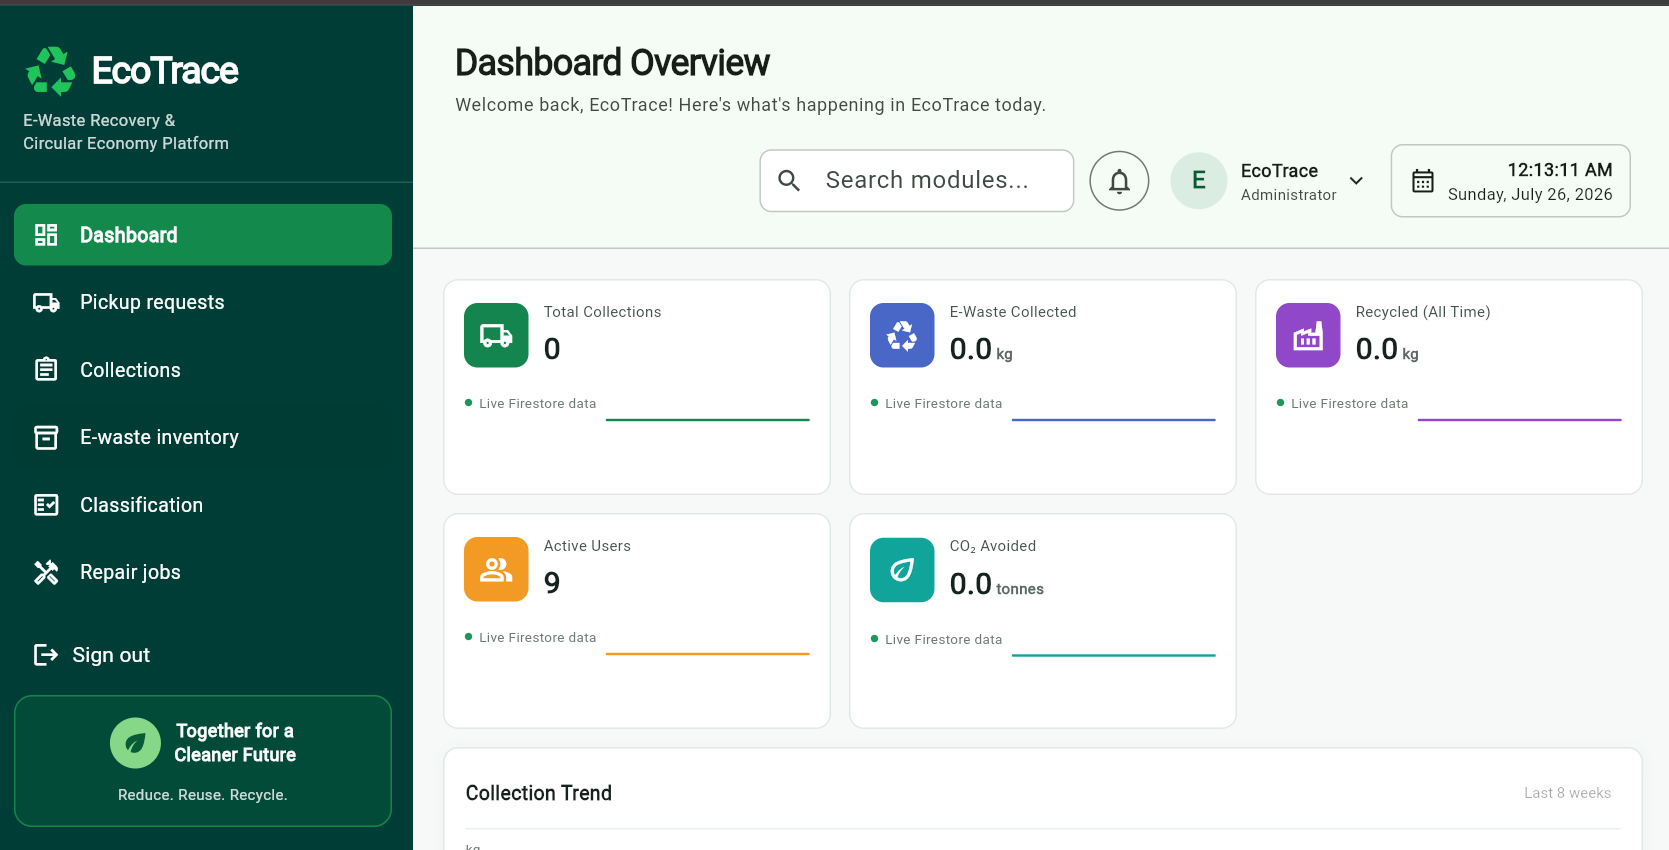
\includegraphics[width=0.85\textwidth]{figures/administrator-dashboard.png}
  \caption{Administrator Dashboard}
  \label{fig:screen-admin}
\end{figure}

\begin{figure}[H]
  \centering
  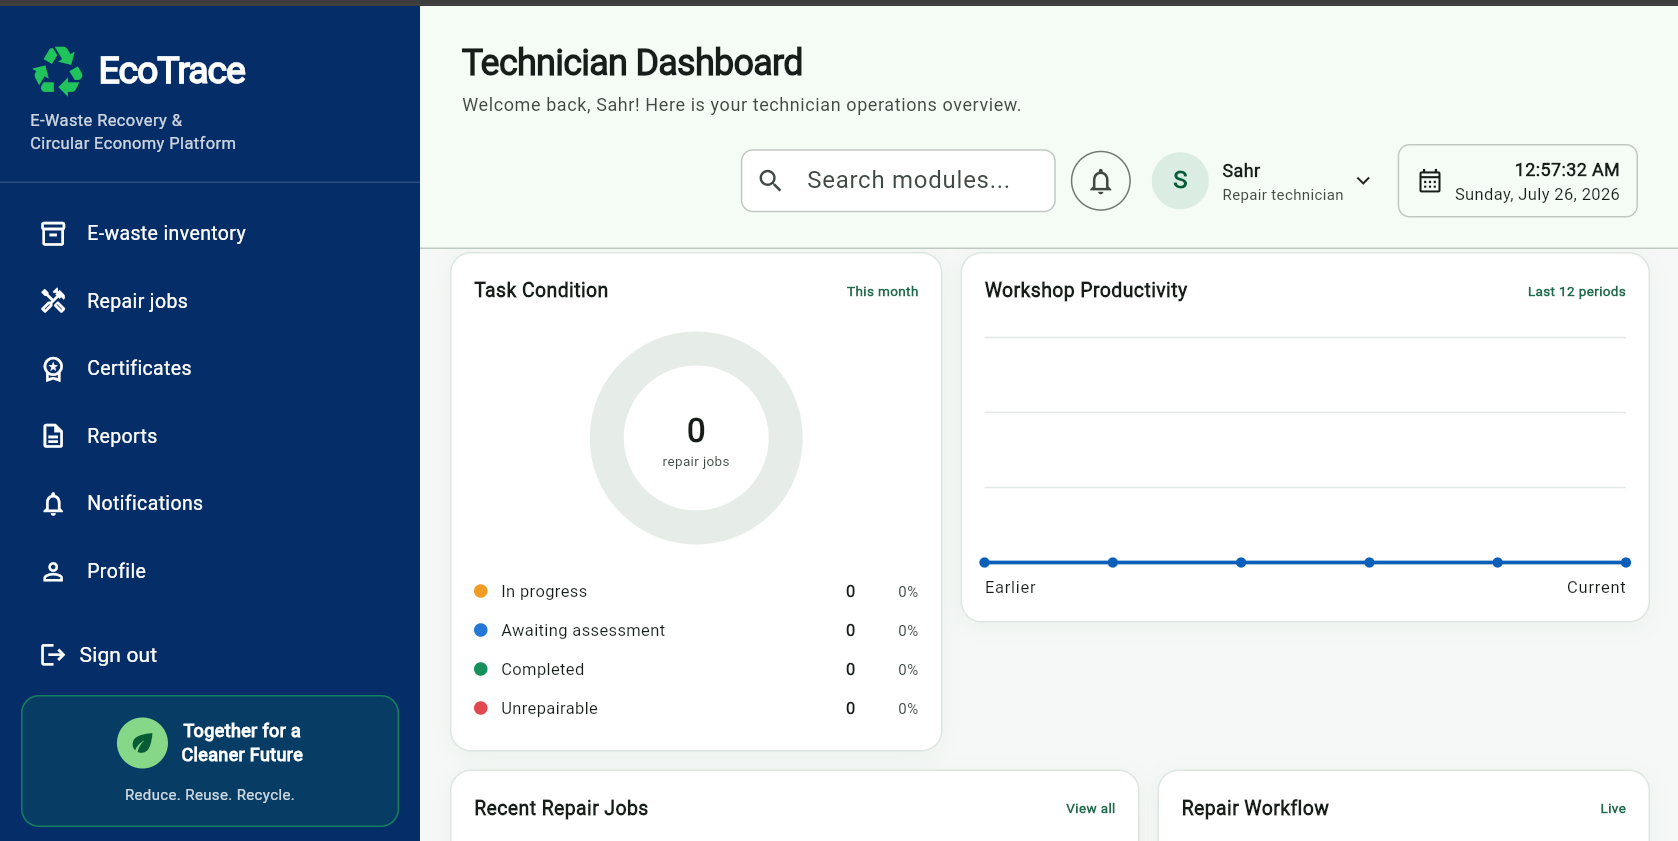
\includegraphics[width=0.85\textwidth]{figures/technician-dashboard.png}
  \caption{Technician Dashboard}
  \label{fig:screen-technician}
\end{figure}

\begin{figure}[H]
  \centering
  \imageplaceholder{Pickup Request screen, showing category/quantity/photo/weight/condition/location/date fields}
  \caption{New Pickup Request Screen}
  \label{fig:screen-pickup}
\end{figure}

\begin{figure}[H]
  \centering
  \imageplaceholder{Monime payment screen, showing provider picker, phone number field, and Pay button}
  \caption{Mobile Money Payment Screen}
  \label{fig:screen-payment}
\end{figure}

\begin{figure}[H]
  \centering
  \imageplaceholder{Payment status screen showing the USSD code and live-updating status}
  \caption{Payment Confirmation Screen}
  \label{fig:screen-payment-confirm}
\end{figure}

\textit{Figures~\ref{fig:screen-login}--\ref{fig:screen-technician} are the
project's own captured screenshots. Figures~\ref{fig:screen-pickup}--\ref{fig:screen-payment-confirm}
are placeholders pending fresh screenshots of the pickup-payment flow added
during this project; the remaining role dashboards (Household/Business,
Driver, Recycler, Environmental Officer, Super Administrator) and feature
screens follow the same placeholder convention and are not reproduced here
for brevity.}

\section{Testing}
\label{sec:testing}

Testing was performed continuously during development, consistent with the
Agile methodology described in Section~\ref{sec:system-design}, and
culminated in a full, real, end-to-end verification of the payment module --
including against Monime's live production environment with real money --
rather than sandbox testing alone. Table~\ref{tab:test-cases} reports the test
cases that have concrete, reproducible evidence; any test not actually
performed is marked \texttt{[TO BE VERIFIED]} rather than claimed.

\begin{longtable}{@{}p{1.1cm}p{2.6cm}p{4.4cm}p{4.4cm}p{1.4cm}@{}}
\caption{Functional and Integration Test Cases} \label{tab:test-cases} \\
\toprule \textbf{ID} & \textbf{Module} & \textbf{Test Case} & \textbf{Actual Result} & \textbf{Status} \\ \midrule
\endfirsthead
\toprule \textbf{ID} & \textbf{Module} & \textbf{Test Case} & \textbf{Actual Result} & \textbf{Status} \\ \midrule
\endhead
T-01 & Payment & Create a Monime Payment Code with both a provider and a phone number restriction set & Monime rejected with \texttt{400 arguments\_invalid}, reproduced independently three times, isolating the exact cause & Pass (bug found) \\
T-02 & Payment & Create a Payment Code with provider restriction only & \texttt{200}, valid USSD code returned & Pass \\
T-03 & Payment & Create a Payment Code with phone restriction only & \texttt{200}, valid USSD code returned, Monime inferred the network from the MSISDN & Pass \\
T-04 & Payment & Complete a sandbox payment via Monime's USSD Simulator (Orange Money) & Webhook delivered \texttt{payment\_code.completed}; backend re-verified against Monime's API; Firestore transaction flipped to \texttt{confirmed}; Flutter UI updated with no manual refresh & Pass \\
T-05 & Payment & Firestore listener on a citizen's own payment-transaction document & Initially failed silently (permission-denied, no error shown -- UI hung on a spinner) & Fail (bug found) \\
T-05b & Payment & Same test, after adding a \texttt{paymentTransactions} rule to \texttt{firestore.rules} and fixing the screen to surface \texttt{snapshot.hasError} & Listener succeeded; error states now surface a message instead of hanging & Pass (regression fixed) \\
T-06 & Payment & Live (real-money) payment: real pickup, real Orange Money account, real Monime live token & SMS and Monime-side insufficient-funds rejection received on first attempt (real network behaviour, not a bug); webhook and re-fetch logic exercised against Monime's live environment & Pass \\
T-07 & Payment & Duplicate \texttt{POST~/payments/monime/initiate} for the same pickup while a payment is still \texttt{pending} & Second call returned the existing transaction instead of creating a second Monime payment code & Pass \\
T-08 & Payment & Cancel a pickup after its payment is \texttt{confirmed} & Payment transaction transitioned automatically to \texttt{refundPending} & Pass \\
T-09 & Pickup & Attempt to confirm a draft pickup via the API without a confirmed payment & Rejected with \texttt{402 payment\_required} & Pass \\
T-10 & Pickup & Submit pickup fee amount from client vs. server-recomputed amount & Server-side recomputation from stored pickup data used in all cases; client-supplied amount never trusted & Pass \\
T-11 & Backend & CORS request from an origin not in \texttt{API\_ALLOWED\_ORIGINS} & Rejected (allow-list enforced app-wide via a single Express middleware ahead of all routes) & Pass \\
T-12 & Backend & Deploy health check (\texttt{GET~/health}) after a Render redeploy & \texttt{200~OK} & Pass \\
T-13 & Frontend build & Grep the compiled Flutter Web output and full \texttt{lib/} source for any Monime credential pattern & No match found in either & Pass \\
T-14 & Authentication & Sign in with a suspended/disabled account & Rejected by \texttt{authenticate} middleware before reaching any route logic & \texttt{[TO BE VERIFIED]} against a real suspended test account \\
T-15 & Cross-platform & Web build (\texttt{flutter build web}) and Android build (\texttt{flutter build apk}) with the payment module included & Both built successfully with no analyzer errors & Pass \\
\bottomrule
\end{longtable}

\subsection{Security Testing}

\begin{itemize}
  \item \textbf{Secrets isolation.} Confirmed by direct search (T-13): no
    Monime token, Firebase service-account key, or Cloudinary secret appears
    in Flutter source or build output. All such secrets live only in Render's
    environment-variable store for the backend services.
  \item \textbf{Amount tampering.} The pickup fee and payment amount are
    always recomputed server-side from the pickup's own Firestore record
    (T-10); the amount field shown in the Flutter payment form is read-only
    and cannot influence what Monime is asked to charge.
  \item \textbf{Webhook trust boundary.} The Monime webhook endpoint is
    intentionally unauthenticated (Monime calls it directly, not a signed-in
    app user), but it never writes anything based on the webhook payload
    alone -- it re-fetches the authoritative status from Monime's API first
    (Section~\ref{sec:payment-module}). This was a deliberate mitigation
    adopted specifically because Monime's webhook-signature scheme could not
    be verified (documented honestly, not silently, in
    Section~\ref{sec:payment-module}).
  \item \textbf{Firestore access control.} Verified that a collection with no
    explicit rule in \texttt{firestore.rules} is completely inaccessible (the
    catch-all deny-by-default), and that this is not merely theoretical: it is
    exactly what caused, and was fixed during, T-05/T-05b above.
  \item \textbf{Idempotency.} Verified (T-07) that a duplicated payment
    initiation request cannot create a second charge for the same pickup.
\end{itemize}

\subsection{System Output}

The completed system was exercised through its own live infrastructure
rather than only a local development build: the Express backend
(\texttt{ecotrace-api}) and the FastAPI notification service
(\texttt{ecotrace-notifications}) both run as deployed Render Web Services,
the Flutter Web build is served from Firebase Hosting, and the Android APK
was built and installed for device testing. The clearest demonstrated output
of the system is the payment module's full loop: a citizen submits a pickup
request, is shown a server-computed fee, selects Orange Money or Afrimoney,
receives a real Monime USSD code, completes payment on a real or simulated
phone, and watches the pickup automatically move from \texttt{draft} to
\texttt{submitted} in real time, with no page refresh and no polling -- output
that was reproduced multiple times during this project, including once
against Monime's live environment with real money.

\section{Chapter Summary}

This chapter documented the implementation of EcoTrace exactly as
delivered, including the specific points where the delivered system departed
from the design proposed in Chapter~\ref{ch:analysis-design}: an
Express/TypeScript backend in place of FastAPI/Python; on-device GPS
capture in place of Google Maps Platform; a pluggable heuristic/external
classifier in place of a bundled PyTorch model; and a Monime mobile-money
payment module added beyond the original design. Every one of these
departures is a deliberate, working decision, not an omission -- and the
payment module in particular was tested more thoroughly than any other part
of the system, against Monime's real sandbox and, briefly, its real production
environment. Chapter~\ref{ch:conclusion} draws conclusions from this
implementation and evaluates the project against its original objectives.